
\documentclass{beamer}
\hypersetup{pdfpagemode=FullScreen} %full screen mode
\setbeamertemplate{navigation symbols}{}
\usepackage[english]{babel} %designed for typesetting lebels(addr lebel,sticky lebels,etc)
\usepackage[latin1]{inputenc} %Accept different input encodings
\usepackage{amsmath,amssymb} 
\usepackage[T1]{fontenc} %for font encoding
\usepackage{times} % use times font instead of default
\usepackage{curves} %for drawing curves
\usepackage{verbatim} %paragraph making environment 
\usepackage{multimedia} %for multimedia like animation,movie etc...
\usepackage{mathptmx} % font style
\usepackage{graphicx} % Allows including images
\usepackage{booktabs} % Allows the use of \toprule, \midrule and \bottomrule in tables
\usepackage{hyperref}
\usepackage{xcolor}
\usepackage{multicol}
\usepackage{algorithm,algorithmic}
\renewcommand{\algorithmicrequire}{\textbf{Input:}}
\renewcommand{\algorithmicensure}{\textbf{Output:}}
\usepackage{lipsum}
\setbeamertemplate{caption}[numbered] % For numbering figures



\mode<presentation> {

% The Beamer class comes with a number of default slide themes
% which change the colors and layouts of slides. Below this is a list
% of all the themes, uncomment each in turn to see what they look like.

%\usetheme{default}
%\usetheme{AnnArbor}
%\usetheme{Antibes}
%\usetheme{Bergen}
%\usetheme{Berkeley}
%\usetheme{Berlin}
%\usetheme{Boadilla}
%\usetheme{CambridgeUS}
%\usetheme{Copenhagen}
%\usetheme{Darmstadt}
%\usetheme{Dresden}
%\usetheme{Frankfurt}
%\usetheme{Goettingen}
%\usetheme{Hannover}
%\usetheme{Ilmenau}
%\usetheme{JuanLesPins}
%\usetheme{Luebeck}
\usetheme{Madrid}
%\usetheme{Malmoe}
%\usetheme{Marburg}
%\usetheme{Montpellier}
%\usetheme{PaloAlto}
%\usetheme{Pittsburgh}
%\usetheme{Rochester}
%\usetheme{Singapore}
%\usetheme{Szeged}
%\usetheme{Warsaw}

% As well as themes, the Beamer class has a number of color themes
% for any slide theme. Uncomment each of these in turn to see how it
% changes the colors of your current slide theme.

%\usecolortheme{albatross}
%\usecolortheme{beaver}%this one also
%\usecolortheme{beetle}
%\usecolortheme{crane} % also use this one
%\usecolortheme{dolphin}
%\usecolortheme{dove}
%\usecolortheme{fly}
%\usecolortheme{lily}
%\usecolortheme{orchid}
%\usecolortheme{rose}
%%\usecolortheme{seagull}
\usecolortheme{crane}
%\usecolortheme{whale} % Best one
%\usecolortheme{wolverine} %use can use this also

%\setbeamertemplate{footline} % To remove the footer line in all slides uncomment this line
%\setbeamertemplate{footline}[page number] % To replace the footer line in all slides with a simple slide count uncomment this line

%\setbeamertemplate{navigation symbols}{} % To remove the navigation symbols from the bottom of all slides uncomment this line
}

\usepackage{graphicx} % Allows including images
\usepackage{booktabs} % Allows the use of \toprule, \midrule and \bottomrule in tables
\setbeamercovered{transparent}
\setbeamertemplate{bibliography item}[text]
\setbeamertemplate{theorems}[numbered]
\setbeamerfont{title}{size=\Large}%\miniscule,command,tiny, scriptsize,footnotesize,small,normalsize,large,Large,LARGE,huge,Huge,HUGE
\setbeamerfont{date}{size=\tiny}%{\fontsize{40}{48} \selectfont Text}

\setbeamertemplate{itemize items}[ball] % if you want a ball
\setbeamertemplate{itemize subitem}[circle] % if you wnat a circle
\setbeamertemplate{itemize subsubitem}[triangle] % if you want a triangle


%------------------customized frame----------------------------
\newcounter{cont}

\makeatletter
%allowframebreaks numbering in the title
\setbeamertemplate{frametitle continuation}{%
   % \setcounter{cont}{\beamer@endpageofframe}%
    %\addtocounter{cont}{1}%
   % \addtocounter{cont}{-\beamer@startpageofframe}%
   % (\insertcontinuationcount/\arabic{cont})%
}
\makeatother
%-----------------------customized-----------------------------




%----------------------------------------------------------------------------------------
%	TITLE PAGE
%----------------------------------------------------------------------------------------

\title[SIAM]{Impresi\'on 3D: Un mundo inexplorado} % The short title appears at the bottom of every slide, the full title is only on the title page

%\author[AKS]{Ajit Kumar Sahoo \texorpdfstring{\scriptsize Regd No: 16MCPC03}{}}

\institute[UTFSM] % Your institution as it will appear on the bottom of every slide, may be shorthand to save space
{


%\begin{center}
%\includegraphics[width=0.1\textwidth]{uoh.png}
%\end{center}
\vspace{2cm}
\medskip

Mat\'ias Mart\'inez\\% Your institution for the title page

%\medskip
%\textit{john@smith.com} % Your email address
}
%This will place the image at position "30 right/left and 120 up/down" relative to the top left corner of the current page.
\titlegraphic{%
  \begin{picture}(0,0)
    \put(30,125){\makebox(0,0)[rt]{
\includegraphics[width=2cm]{logo.png}}}
  \end{picture}}
 \date{\today} % Date, can be changed to a custom date
\begin{document}

\begin{frame}
\titlepage % Print the title page as the first slide
\end{frame}
\begin{frame}
  \frametitle{\'Indice}
 % \tableofcontents[pausesections,shaded]
 \tableofcontents
\end{frame}
% TABLE OF CONTENTS AT BEGIN OF EACH SECTION
\AtBeginSection[]{
  \begin{frame}<beamer>
    \frametitle{Indice}
   \tableofcontents[currentsection]
  \end{frame}}
%----------------------------------------------------------------------------------------
%	PRESENTATION SLIDES
%----------------------------------------------------------------------------------------


%-------------------------------------------------------------------------------
%-------------------------------INTRODUCTION--------------------------------
%-----------------------------------------------------------


\section{?`Qu\'e es y c\'omo funciona la impresi\'on 3D?} 
\begin{frame}[allowframebreaks]
\frametitle{?`Qu\'e es y como funciona la impresi\'on 3D?}
\begin{itemize}
    \item 
Existen varios tipos de impresi\'on pero las principales son la impresi\'on de resina y la FDM (Fused deposition modeling)\\
\item Normalmente los archivos imprimibles son del tipo .obj .stl 3mf.\\
\item Adem\'as estos archivos tienen que pasar por un programa conocido como slicer o laminador, este puede ser el que sea de tu preferencia, los mas usados son Cura y Prusa.
\end{itemize}
\end{frame}

\begin{frame}{Ejemplos}
\centering
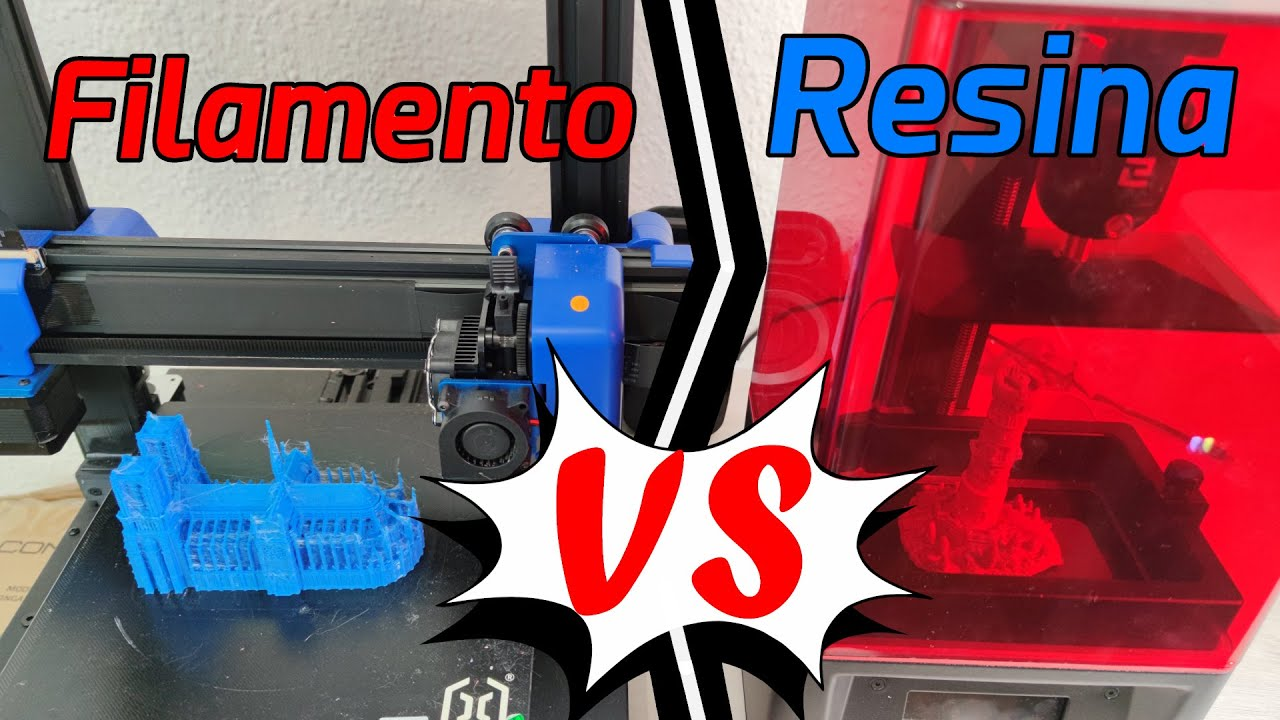
\includegraphics[width=10cm]{maxresdefault.png}
\end{frame}
\begin{frame}{Otros Ejemplos}
    \centering
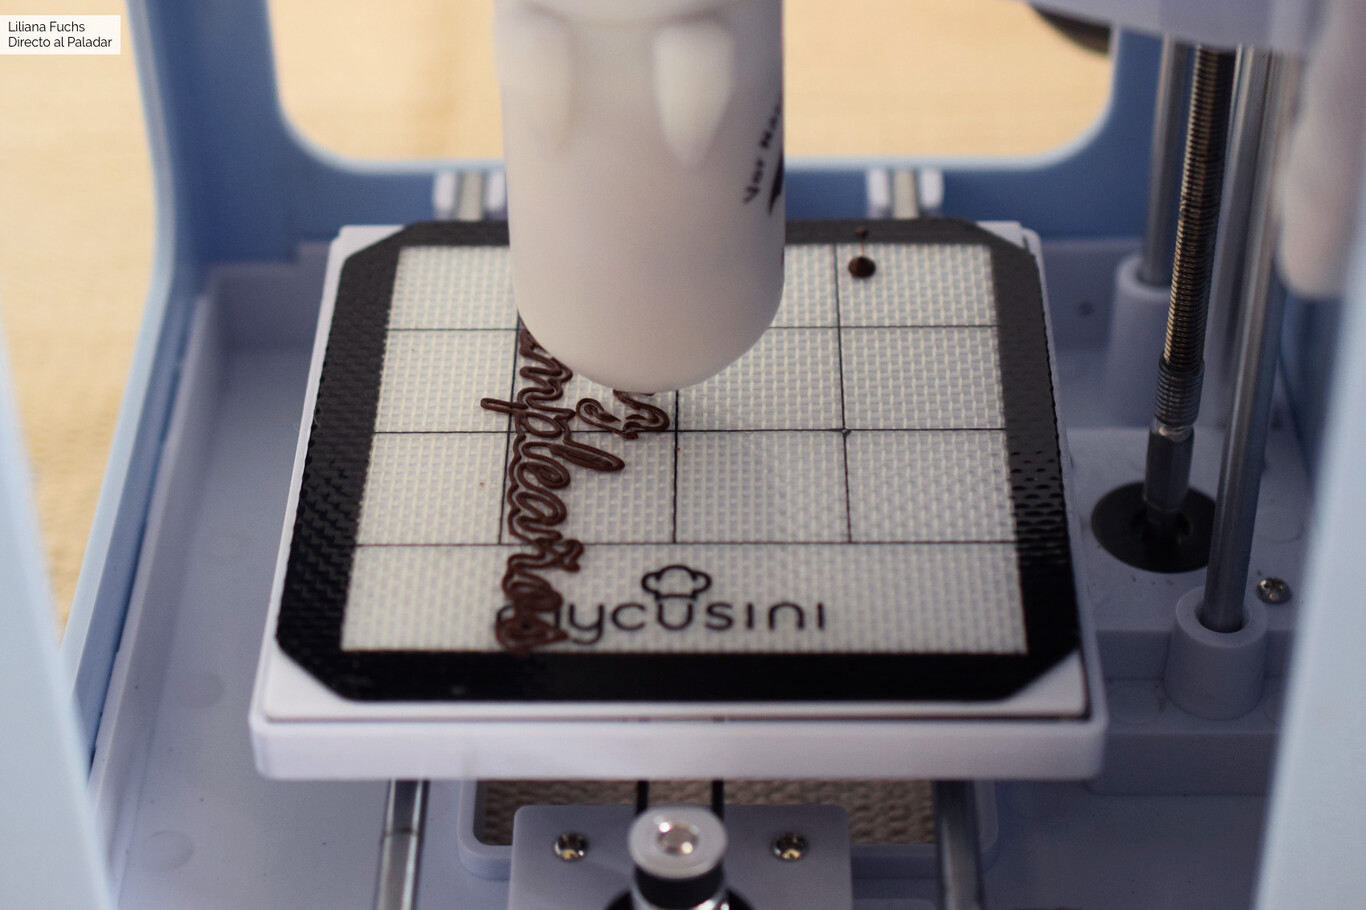
\includegraphics[width=10cm]{1366_2000.png}
\end{frame}
\begin{frame}{Otros Ejemplos}
    \centering
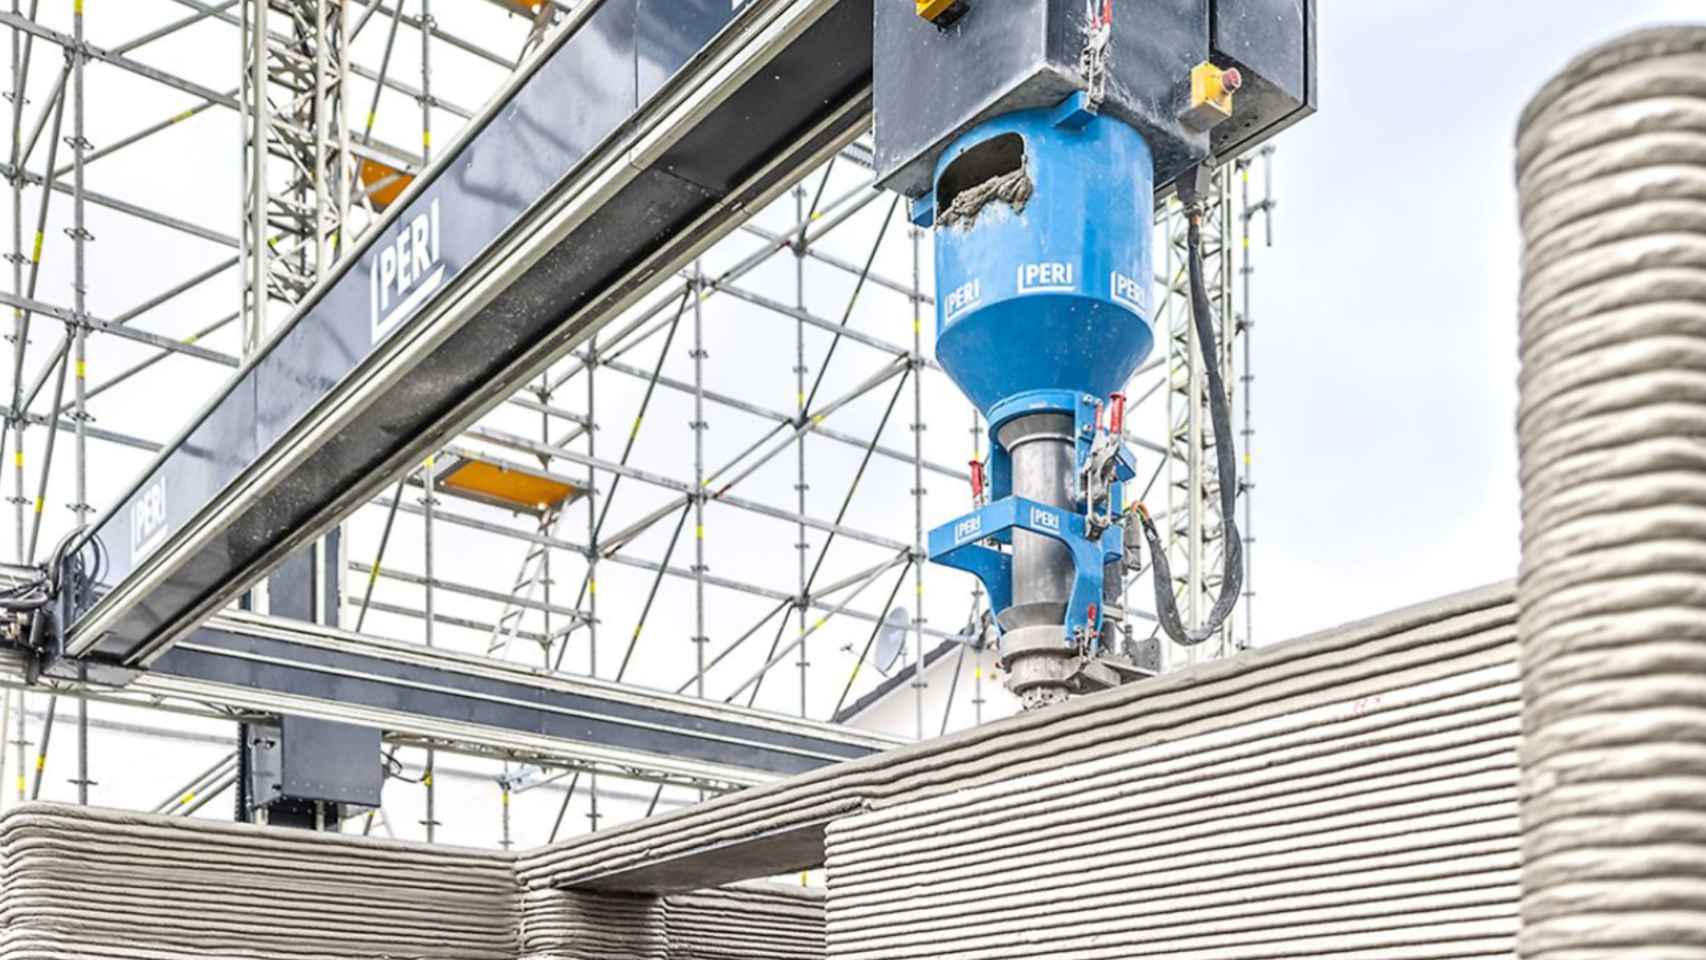
\includegraphics[width=10cm]{tecnologia-impresion_3d-tecnologia_538707966_165982583_1706x960.jpg}
\end{frame}



\section{?` C\'omo funciona es el Slicer?}
\begin{frame}[allowframebreaks]
\frametitle{Slicer o Laminador}
Dentro del mundo de la impresi\'on, una vez sabemos que tipo de m\'aquina utilizaremos podemos elegir una variedad de laminadores, entre los mas utilizados se encuentran:
\begin{itemize}
    \item Cura 
    \item Simplify3D
    \item PrusaSlicer
    \item Octoprint
    \item BambuLab
\end{itemize}
\end{frame}

\begin{frame}[allowframebreaks]
\frametitle{Slicer o Laminador}
\begin{itemize}
    \item La principal funci\'on del programa es preparar el gcode, en este tenemos que verificar todas las configuraciones de impresi\'on como: 
    \begin{itemize}
        \item Temperatura.
        \item Soportes.
        \item Densidad de relleno.
        \item Paredes, capas superiores e inferiores.
        \item Material.
        \item Retracci\'on.
        \item Otros.
    \end{itemize} 
\end{itemize}
\end{frame}
\begin{frame}{?` Qu\'e es el gcode?}
    Conjunto de instrucciones que se le entrega a la m\'aquina con el fin de obtener la impresi\'on.
\end{frame}

\begin{frame}{Matem\'aticas}
Spline: El t\'ermino "spline" se utiliza para referirse a una amplia clase de funciones que se utilizan en aplicaciones que requieren interpolaci\'on y/o suavizado de datos. 
\begin{center}
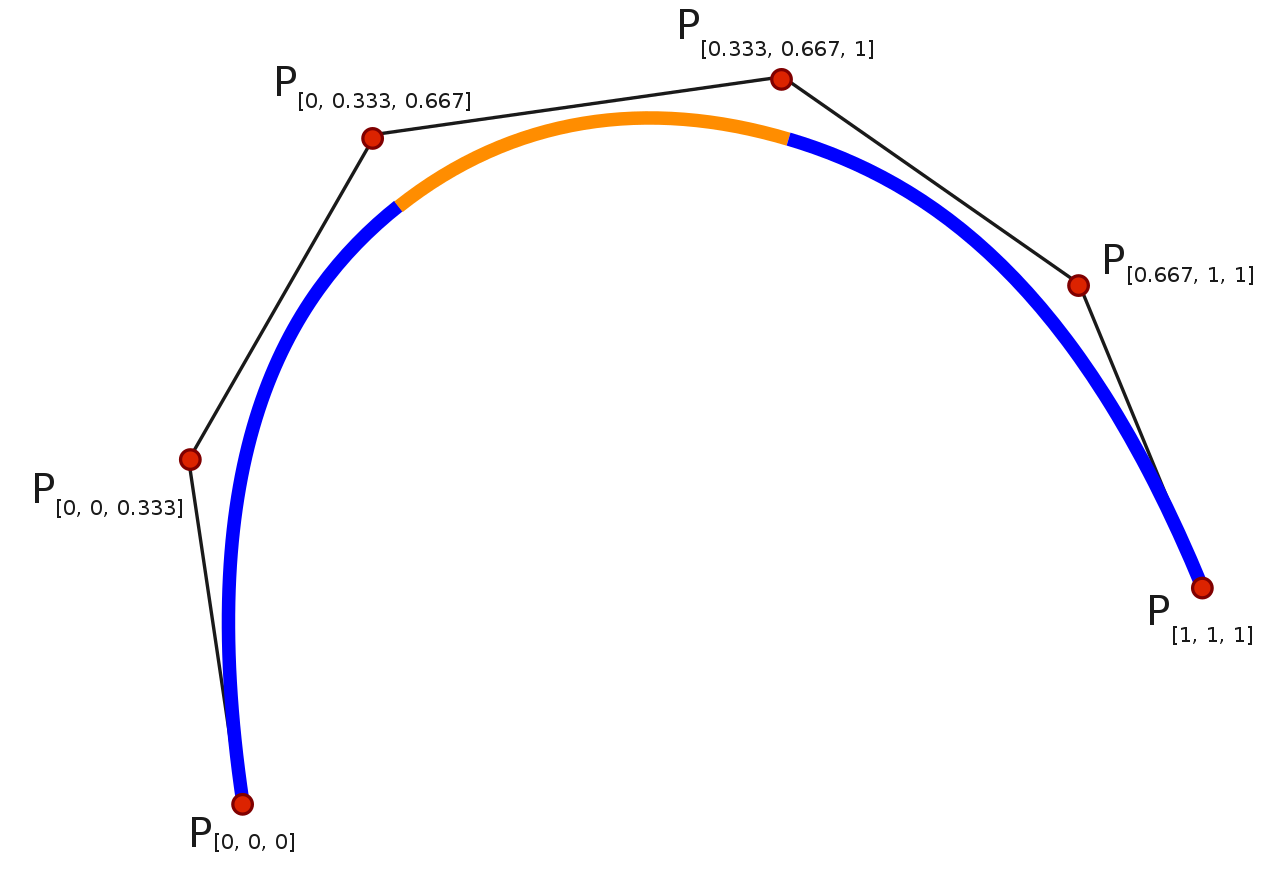
\includegraphics[width=8cm]{1280px-Parametic_Cubic_Spline.svg.png}
\end{center}
    
\end{frame}
\begin{frame}{Matem\'aticas}
    Los datos pueden ser unidimensionales o multidimensionales. Las funciones spline para interpolaci\'on normalmente se determinan como minimizadores de medidas adecuadas de rugosidad (por ejemplo, curvatura cuadr\'atica integral) sujetas a las restricciones de interpolaci\'on.
\end{frame}









\section{Materiales}
\begin{frame}{Tipos de materiales:}
Existen muchos materiales imprimibles pero aqui dejo algunos o los mas comunes.
\begin{itemize}
    \item PLA
    \item PETG
    \item PLA+
    \item TPU
    \item ABS
    \item Resina
    \item Nylon
    \item PVA
\end{itemize}
    
\end{frame}

\begin{frame}{Materiales}
    \begin{itemize}
        \item Cada material cumple con aplicaciones diferentes
        \item Pros:
        \begin{itemize}
            \item PLA: F\'acil de imprimir, es barato, variedad de colores, facil de adquirir, no es t\'oxico
            \item ABS: Resistente a altas temperaturas, mayor dureza
            \item PETG: No es tan complicado de imprimir, es de f\'acil adquisici\'on, se puede conseguir reciclando botellas de pl\'astico, resistente.
            \item TPU: Flexible
        \end{itemize}
        \item Contras:
                \begin{itemize}
            \item PLA: No muy resistente, se deforma a baja temperatura.
            \item ABS: T\'oxico, complejo de imprimir tiene que estar en un ambiente adecuado con buena ventilaci\'on
            \item PETG: No es recomendable imprimirlo en cualquier impresora, muy residual.
            \item TPU: Caro, muy complejo de imprimir pues al ser flexible el material no se comporta muy bien con las temperaturas y la adherencia
        \end{itemize}
        
    \end{itemize}
\end{frame}

%--------------------------------------------------------------------------------------------------------------------------------


%--------------------------------------------------------------------------------------------------------------------------------
%\section{Information processing  issues}
%-----------------------------------------------
%\begin{frame}
%\frametitle{Information processing issues}
%\begin{itemize} 
%\item In collaborative processing
%\begin{itemize}
%\item Target detection, localization, communication, storage, querying...
%\end{itemize}
%\color{lightgray}
%\item  In networking
%\begin{itemize}
%\color{lightgray}
%\item  aggregation, routing, Data naming,...
%\end{itemize}
%\end{itemize}
%\end{frame}
%-----------------------------------------------
%\begin{frame}[fragile] % Need to use the fragile option when verbatim is used in the slide
%\frametitle{Citation}
%An example of the \verb|\cite| command to cite within the presentation:\\~
%Citation \cite{Souza} requires .
%\end{frame}
%------------------------------------------------


%-----------------------------------------------------------------------------------------

%-----------------------------------------------------------------------------------------


%----------------------------------------------------------------------------------------

\end{document}
